\chapter{Conclusões e Trabalho Futuro} \label{chap:concl}

\section*{}

%Neste capítulo é apresentado o plano de trabalho já realizado, que culmina com a elaboração deste relatório, e também o planeamento que será adotado a partir deste momento.
%
%\section{Satisfação dos Objetivos}
%
%Segundo o plano de trabalho apresentado na Figura~\ref{fig:gantt1}, era necessário realizar a revisão do estado da arte e compreender melhor o contexto em que se insere o projeto. Ambas as tarefas deviam convergir numa clara compreensão do problema, na apresentação de uma perspetiva de solução, cuja implementação deverá ser iniciada a partir desta etapa, e finalmente na escrita do presente relatório. Para além disso, foram realizadas também duas apresentações (de 5 e 10 minutos, respetivamente) para exposição do tema da dissertação e de uma visão global do estado da arte, bem como uma possível solução para o problema proposto.
%\\Tendo em conta os resultados obtidos e relatados neste documento, considera-se que foram cumpridas atempadamente as obrigações do plano elaborado, assim como foram atingidos todos os objetivos inerentes.
%
%\section{Trabalho Futuro}
%
%O trabalho continuará a ser desenvolvido segundo as etapas e datas previstas no plano de trabalho que se descreve na Figura~\ref{fig:gantt2}.
%\\De acordo com o plano traçado em conjunto com a OPT e a STCP, será apresentado um primeiro protótipo já no início do mês de março, sendo depois realizados testes com utilizadores reais na rede de autocarros da STCP. Neste primeiro protótipo estarão apenas algumas funcionalidades desenvolvidas, sendo elas:
%\begin{itemize}
%\item Possibilidade de registo e autenticação (ainda sem dados de pagamento);
%\item Possibilidade de comprar títulos de viagem (feito com saldo inicialmente atribuído);
%\item Possibilidade de validar títulos de viagem;
%\item Possibilidade de verificação por parte do revisor;
%\item Possibilidade de visualização de saldo da carteira virtual e da carteira de títulos de viagem;
%\item Possibilidade de consulta de histórico de operações.
%\end{itemize}
%
%Após o término da fase de testes, serão realizados inquéritos e entrevistas de modo a recolher a opinião dos sujeitos de teste, tendo em vista o melhoramento das funcionalidades implementadas, quer a nível de usabilidade como correção de falhas.
%\\Segue-se então a realização do segundo protótipo, com todas as funcionalidades descritas no Capítulo~\ref{chap:chap3} e as alterações que se acharem convenientes após a análise dos inquéritos e entrevistas. Tal como o primeiro protótipo, este será também sujeito a um período de testes com utilizadores reais em contexto real, sendo depois recolhidas opiniões e sugestões de melhoramento.
%\\A fase seguinte será a elaboração de recomendações para os operadores de transportes públicos de passageiros, tendo em vista a introdução destes serviços nos seus produtos.
%\\Por fim, a escrita do relatório final da dissertação que reunirá toda a informação recolhida e produzida no âmbito da dissertação.
%
%\begin{figure}[t]
%  \begin{center}
%    \leavevmode
%    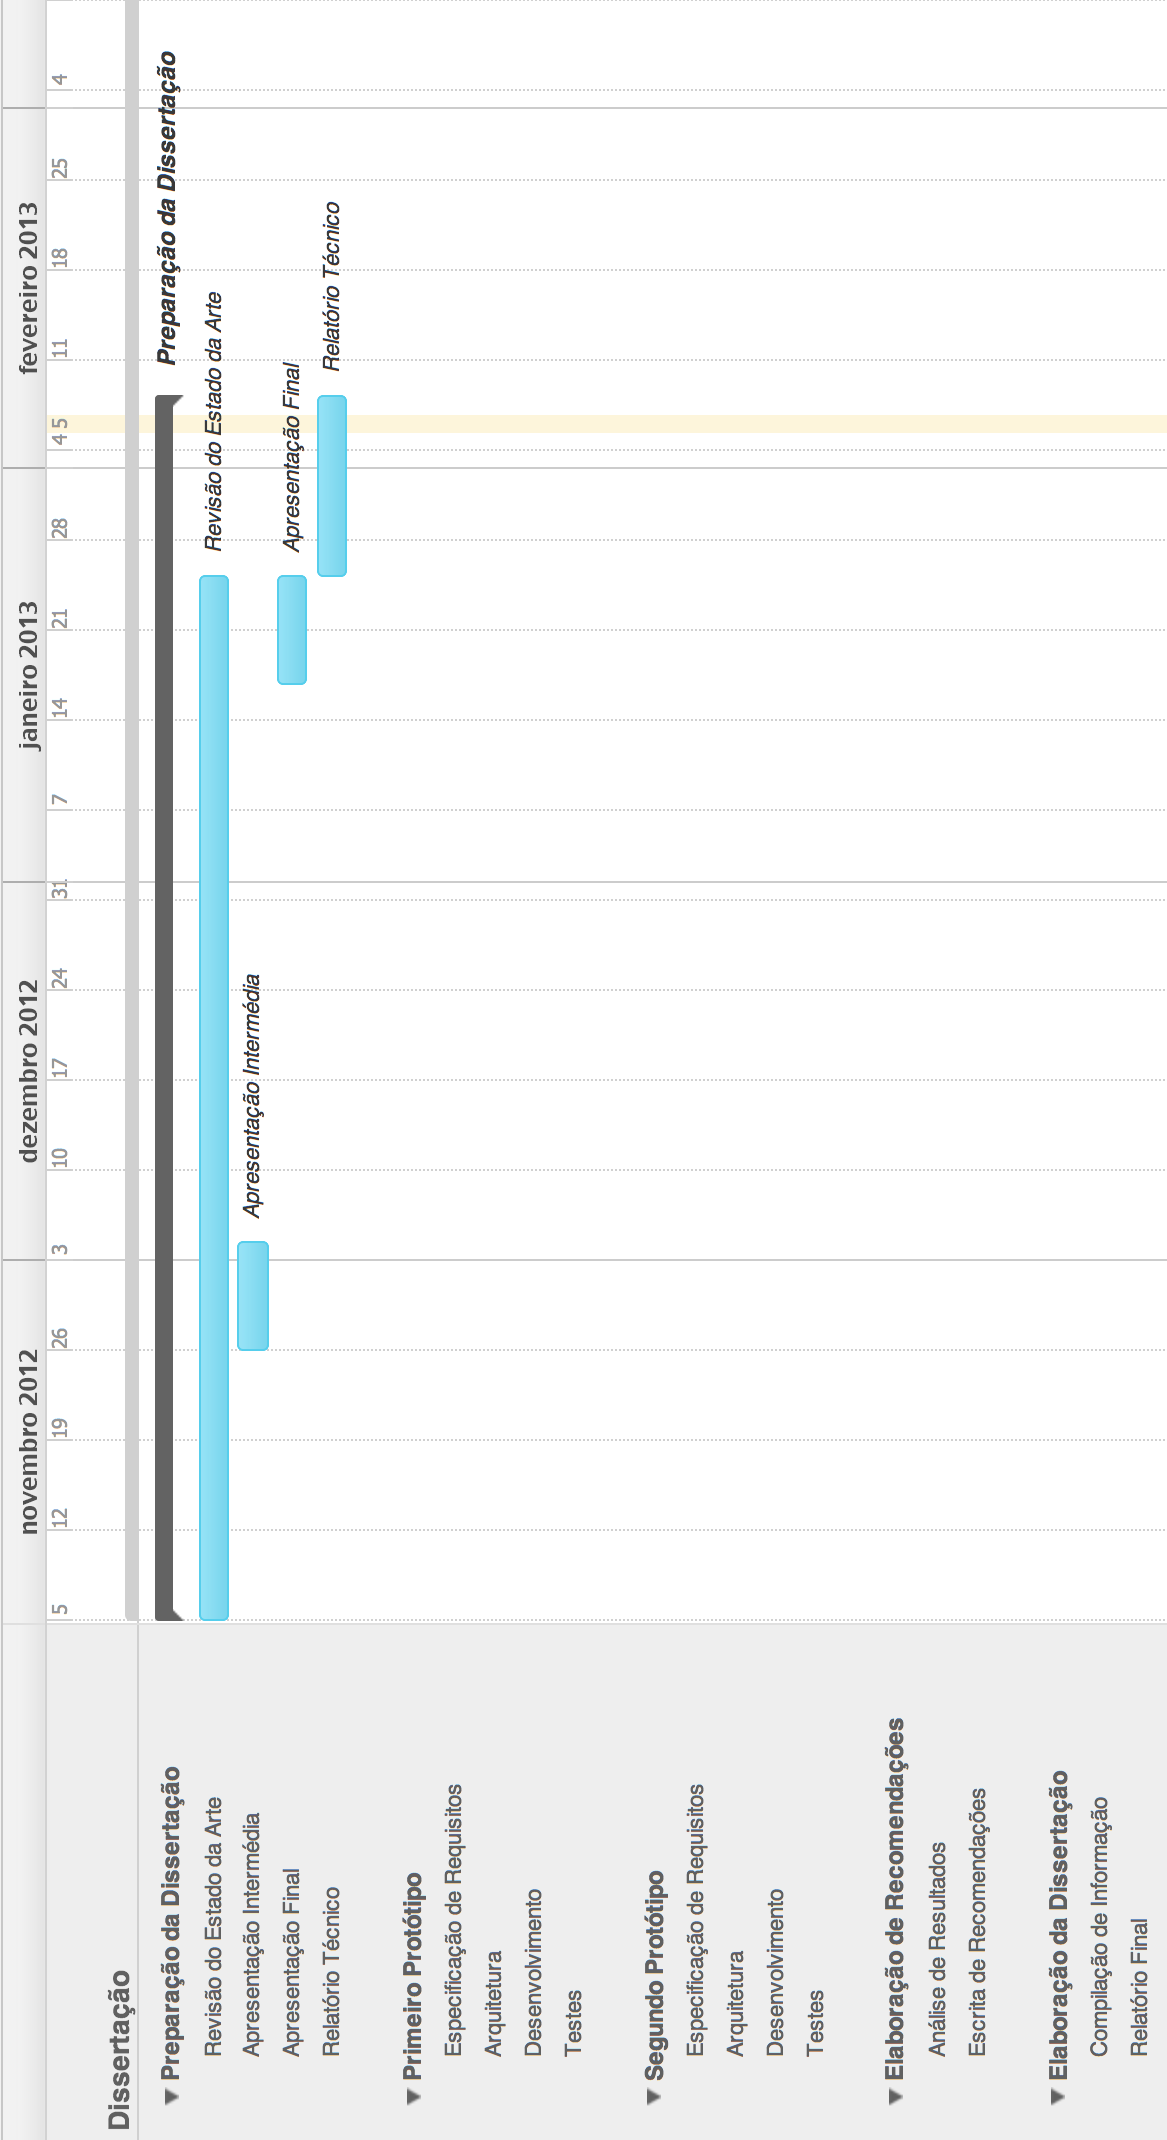
\includegraphics[height=23cm]{gantt_part1}
%    \caption{Planeamento da primeira fase da dissertação}
%    \label{fig:gantt1}
%  \end{center}
%\end{figure}
%
%\begin{figure}[t]
%  \begin{center}
%    \leavevmode
%    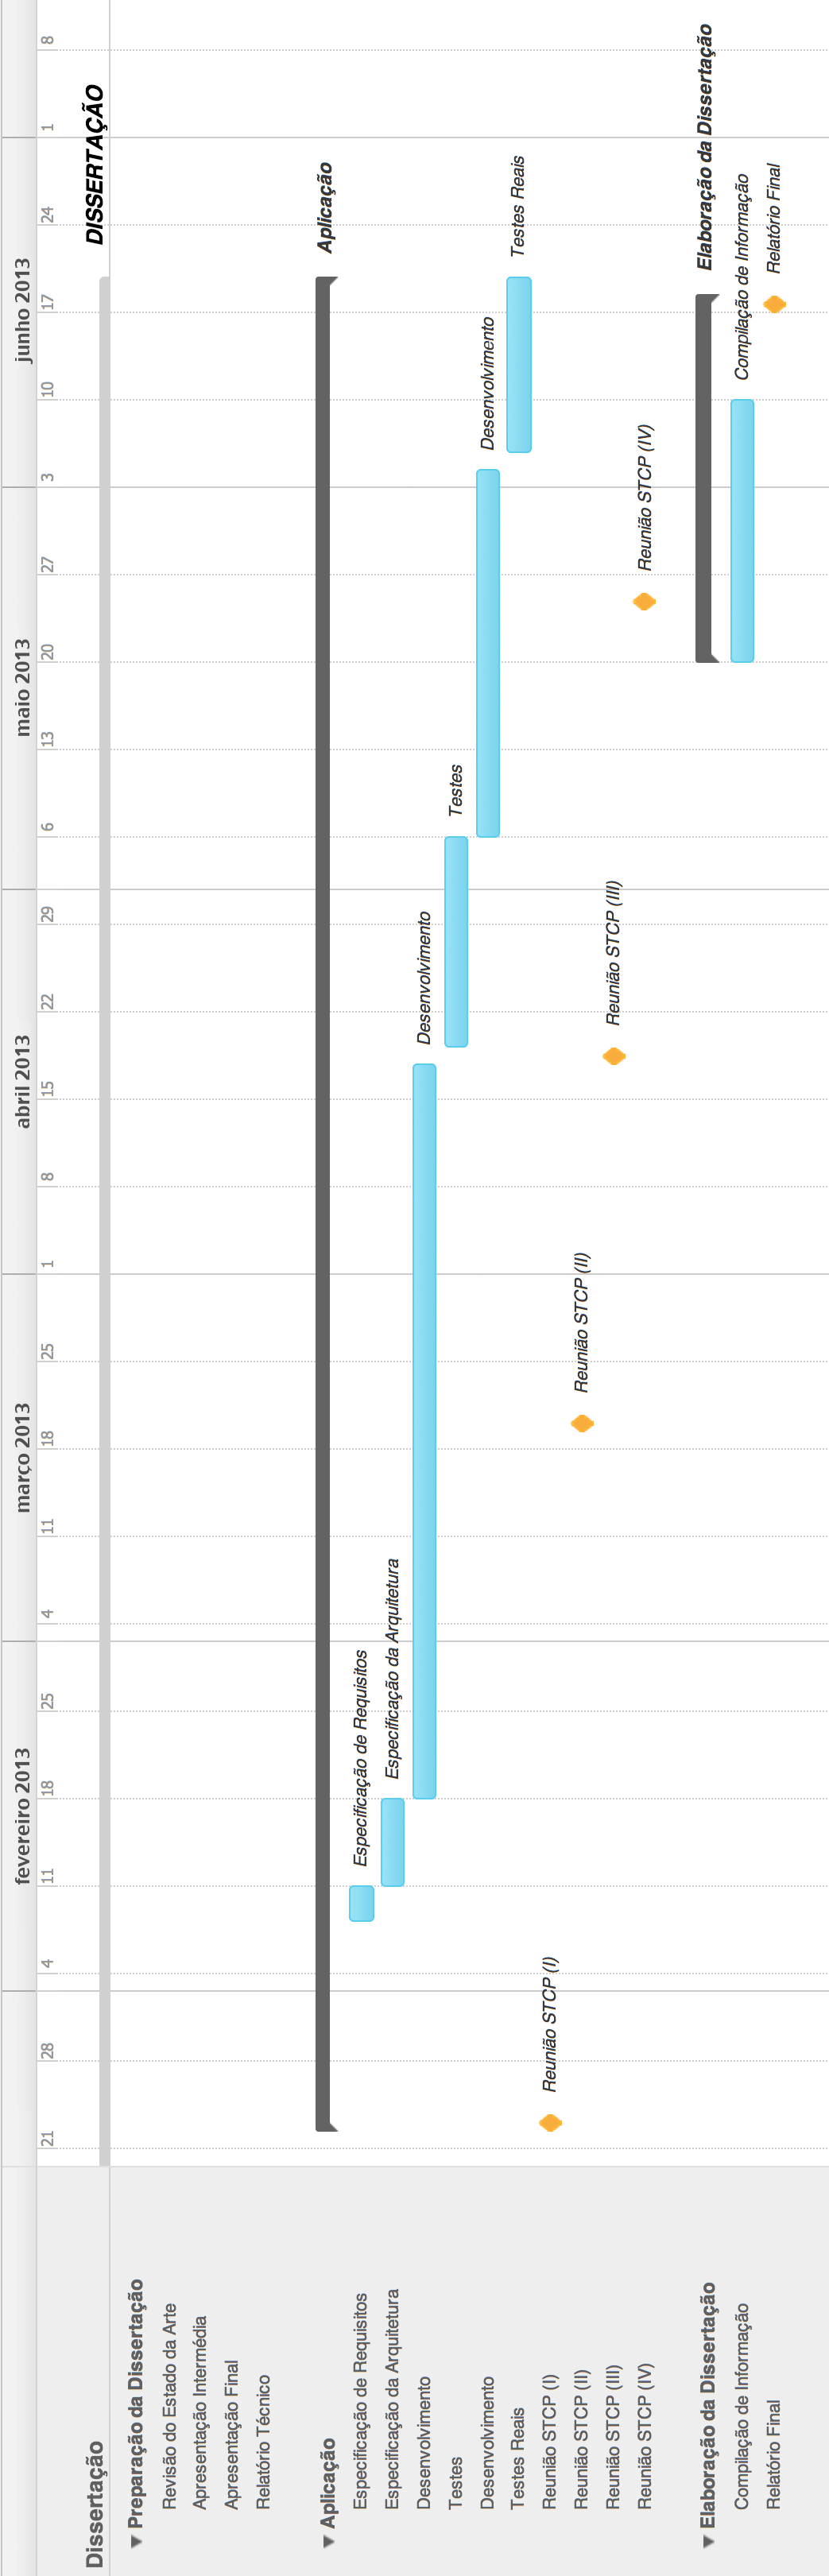
\includegraphics[height=23cm]{gantt_part2}
%    \caption{Planeamento da segunda fase da dissertação}
%    \label{fig:gantt2}
%  \end{center}
%\end{figure}